\documentclass[dvipsnames,border=3pt]{standalone}
\usepackage{tikz}
\usetikzlibrary{arrows}
\usetikzlibrary{shapes}
\usepackage{enumitem}
\usepackage{bm}
\usepackage{mathdots}
\usepackage{amsmath}
\usetikzlibrary{shadings}
\usetikzlibrary{decorations.pathreplacing}
\usepackage{helvet}
\usetikzlibrary{arrows.meta}
\usepackage{graphicx}
\usepackage{pgfplots}
\usepackage{pgfplotstable}
\usepackage{filecontents}
\usetikzlibrary{plotmarks}
\pgfplotsset{compat=newest}

\renewcommand{\familydefault}{\sfdefault}

\definecolor{mylightgray}{cmyk}{0,0,0,0.1}
\usetikzlibrary{arrows,decorations.pathmorphing,backgrounds,fit,positioning,shapes.symbols,chains}

\begin{document}

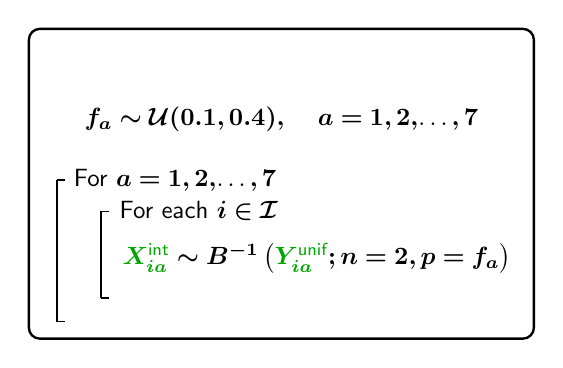
\begin{tikzpicture}
    % trim=left botm right top
    
    \node[draw, rounded corners=4, line width=0.3mm, text width=6.18cm, text height=3.7cm] at (9.55,-9.25) {};
    %\node[circle,draw,line width=0.2mm,xscale=1.2,yscale=1.2,fill=GreenYellow] at (7,-7.6) {};
    %\node at (7,-7.6) {\textbf{5}};
    
    \node[xscale=0.9,yscale=0.9] at (9.55,-8.43) {\bm{$f_a \sim \mathcal{U}(0.1,0.4),$} \quad \bm{$a = 1,2, $}$\dots$\bm{$,7$}};
    
    \node[xscale=0.9,yscale=0.9] at (8.2,-9.2) {For \bm{$a = 1,2, $}$\dots$\bm{$,7$}};
    \node[xscale=0.9,yscale=0.9] at (8.5,-9.6) {For each \bm{$i \in \mathcal{I}$}};
    
    \node[xscale=0.9,yscale=0.9] at (10,-10.2) {\bm{$\textcolor{black!35!green}{X^\text{int}_{ia}} \sim B^{-1}\left(\textcolor{black!35!green}{Y^\text{unif}_{ia}};n=2,p=f_a\right)$}};
    
    \draw[line width=0.2mm] (6.7,-9.2) -- (6.7,-11);
    \draw[line width=0.2mm] (6.7,-9.2) -- (6.8,-9.2);
    \draw[line width=0.2mm] (6.7,-11) -- (6.8,-11);
    
    \draw[line width=0.2mm] (7.26,-9.6) -- (7.26,-10.7);
    \draw[line width=0.2mm] (7.26,-9.6) -- (7.36,-9.6);
    \draw[line width=0.2mm] (7.26,-10.7) -- (7.36,-10.7);

    \end{tikzpicture}
    
\end{document}